\chapter{The lattice-Boltzmann method}\label{sec:lbm}
Rather than modelling on a macroscopic or microscopic scale, the
lattice-Boltzmann method (LBM) operates at a scale in between those,
often referred to as a mesoscopic scale. Nowadays, the method is most
frequently used in modelling of fluid dynamics, i.e. computing
solutions of the macroscopic Navier-Stokes equations. However, the
lattice-Boltzmann method is not limited to this case and may be used
to model other macroscopic systems as well. In this chapter a LBM
approach will, in addition to the Navier-Stokes equations, also be
formulated for the Nernst-Planck and Poission's equation.

\nomenclature{LBM}{Lattice-Boltzmann Method}

\section{Historical overview}
With the introduction of electronic calculating machines came also
completely new possibilities of tackling difficult problems. New
fields of computational science was born and methods for solving both
new and traditional problems were developed.

The idea of using a discrete and simplified version of the
Boltzmann-equation dates back to the mid 60's \cite{scholarpedia-lbm}
with an experimental attempt to model simple gas dynamics. However, at
the time, this kind of statistical computational approaches was not
considered a serious alternative for the modelling of more
sophisticated and complex systems such as fluid behaviour. It was
first in the mid 80's when Frisch, Hasslacher and Pomeau showed that a
lattice automaton that conserved mass and momentum in the collisions
and with a lattice of certain symmetry, reproduced the Navier-Stokes
equations in a macroscopic limit. It was by their work and the always
increasing computational power that made the idea of fluid modelling
on a mesoscopic scale a serious research topic. \cite{wolf-gladrow}

The lattice gas automata (LGA) approach was not perfect and suffered
from some notable flaws, e.g. that the boolean nature of the method
introduced statistical noise and that lack of symmetry in the lattices
used made the advection non-isotropic. The statistical noise was
usually dealt with by averaging which resulted in a coarsed domain and
the advection issue was handled by introducing lattices of higher
symmetry. An other consequence of the boolean variables is that only one
particle per state was allowed which resulted in an equilibrium state
from Fermi-Dirac statistics rather than the desired Maxwell-Boltzmann
statistics. 

As the flaws of the LGA approach was resolved one by
another, the method evolved into what we today know as the
lattice-Boltzmann method, with the crucial refinement of using
continuous distributions over boolean variables. \cite{wolf-gladrow}

Today, the lattice-Boltzmann method is in many situations indeed a
competitor to more traditional CFD methods. For example with
advantages when it comes to parallelisation or implementing boundary
conditions in complex geometries. One major downside with the LBM is
the lack of theoretical work done and lack of literature compared to
the case with more traditional methods such as finite element/volume
methods. \cite{junk-asym}

\nomenclature{LGA}{Lattice Gas Automata/Automaton}
\nomenclature{CFD}{Computational Fluid Dynamics}


\section{Statistical background}\label{sec:lbm:stat}
Consider one litre of air. At STP, the volume will contain in the
order of $10^{22}$ molecules. In order to model this system
microscopically, 6 variables per molecule will be needed to describe
the microstate of the system. Just to store the state of the system in
a computer would require more space than the estimated size of the
whole world wide web times one million \cite{wolfram-alpha-web}. Thus,
for these kind of systems, the microscopic approach is somewhat
impractical.

\nomenclature{STP}{Standard Temperature and Pressure}

Statistical approaches have been developed for these types of
problems. A fundamental quantity used for describing the system is a
continuous probability density distribution, $f$. This distribution
may be regarded as an average over the microstates. Consider a volume
of $d^3\x d^3\mathbf{p}$ in phase space, the number of molecules, $dN$
in this volume is then given through the density distribution, $f$ as

\begin{equation}
dN(\x, \p, t) = f(\x, \p, t)\drm^3\x \drm^3\p.
\end{equation}
Thus $f(\x, \p, t)$ is a measure of the number of particles at
location $\x$ with momentum $\p$ and at time $t$. Macroscopic variables are
obtained by summing, e.g. the particle density, $n$, is obtained from

\begin{equation}
n(\x, t) = \int f(\x, \p, t) \drm^3\p
\end{equation}
and the macroscopic momentum density of the system is determined by

\begin{equation}
\rho(\x, t) \ubf(\x, t) = \int \p f(\x, \p, t) \drm^3\p
\end{equation}
where $\rho = m n$ is the mass density. Multiplying $f$ by a power $k$ of
$\p$ or $\mathbf{v} = \p/m$ and integrating is often referred to as
taking the $k$:th moment of $f$ and is a term that will be used
throughout this chapter.

In the late 19th century, Boltzmann developed a model for the time
evolution of $f$. To do this he had to make several
assumptions. First, only collisions between two particles are
considered, this makes the equation mostly applicable to dilute
gases. Second, the two particles colliding are assumed to be
uncorrelated before the collision. Third, external forces are assumed
not to affect the collisions \cite{wolf-gladrow}. The equation is
named after its father to the Boltzmann (transport) equation and
reads:

\begin{equation}\label{eq:lbm:boltzmann-eq}
\partial_t f + \frac{\p}{m} \cdot \nabla_{\x}f + \frac{\F}{m} \cdot
\nabla_{\mathbf{v}}f = Q(f, f)
\end{equation}
where $f$ is the distribution function for a single species collection
of particles of mass $m$, $\F$ is external forces, $\p$ is momentum,
$\nabla_{\x}$ and $\nabla_{\mathbf{v}}$ are the gradients in location
and velocity space respectively. The right-hand side contains the so
called collision term which in the general case is expressed as an
integral. This integral states how the distribution function changes
after a two particle collision. However, the structure of this
integral is in most physical situations too complicated to be used
directly. Therefore, a number of simplifications have been proposed
during the years.

When designing these approximations, at least two main properties of
the collision integral must be kept. \cite{wolf-gladrow}

\begin{enumerate}
  \item The same quantities that are conserved under collisions in the
    collsion integral must also be conserved in the approximation.
  \item Boltzmann's H-theorem must be fulfilled for the
    approximated collision operator.
\end{enumerate}

Without being to specific, the H-theorem states that the entropy
computed from $f$ is always increasing with time and that the maximum
entropy is obtained for a so called Maxwellian distribution in
momentum/velocity space. Boltzmann used an other quantity denoted by H
closely related to entropy, thus the name of the theorem. The
Maxwellian distribution in two dimensions that $f$ tends towards is
given by

\begin{equation}\label{eq:lbm:maxwell}
f^{(M)}(\x, \mathbf{v}, t) = n \left ( \frac{m}{2 \pi k_B T} \right )
\exp{\left( -\frac{m}{2 k_B T} (\mathbf{v} - \ubf)^2\right)}
\end{equation} 
where $\ubf(\x, t)$ is the mean velocity of the particles in the system and
$n(\x, t)$ is the number of particles at location $\x$. In section
\ref{sec:lbm:col}, one of the most widely used approximations of the
collision integral will be presented.


\section{Basic idea of the LBM}
As previously noted, the lattice-Boltzmann method is a mesoscopic
method. This means that the modelling is neither done on a microscopic
(molecular) level nor by direct solving of the macroscopic equations
involved. The aim, in most situations with the lattice-Boltzmann
method is indeed to solve some macroscopic equation but not
direct. Instead a statistical model is used with various mesoscopic
variables that, in some limit, reproduces the macroscopic
variables. It is also possible to ensure that these variables (to some
extent) fulfil a certain macroscopic equation by using a certain
scheme.

Basically the lattice-Boltzmann method solves a discretised version of
eq. \eqref{eq:lbm:boltzmann-eq} for the distribution functions from
which the macroscopic quantities may be determined. Both the spatial
positions and the velocity space is discretised allowing the
distributions to ``sit'' only at certain positions and to stream to
neighbouring locations only in certain directions. A naive way to
visualise the evolution of $f$ is to consider the distribution
functions at the lattice nodes as pseudo particles that move along the
lattice and collide.

Usually in two dimensions the velocity space is discretised into 9
distinct velocities, more about the choice of lattice is discussed in
section \ref{sec:lbm:lattice}. In this case 9 distribution functions
are needed per node which might correspond to one or two macroscopic
variables but is indeed fewer than the number of variables needed for
a microscopic approach.

The discretised Boltzmann equation is referred to as the
lattice-Boltzmann equation (LBE) and is one of the fundamental corner
stones in the lattice-Boltzmann method, it reads:

\begin{equation}\label{eq:lbm:lbe}
f_i(\x + \cbf_i\delta_t, t + \delta_t) - f_i(\x, t) = \Omega_{ij}(\x, t)
\end{equation}
where $f_i$ denotes the distribution function for direction $\cbf_i$,
$\delta_t$ is the time step and $\Omega_ij$ is the (for now
non-specified) collision operator. An implicit sum over the second
velocity index $j$ is assumed. Various forms of collision operators
exist and will be further discussed in section \ref{sec:lbm:col}.

\subsection{Computational algorithm}
In order to solve eq. \eqref{eq:lbm:lbe} the distribution functions
must be set to some initial value. The choice of initial value is in
most cases crucial with respect to stability and accuracy of the
method. More about the initialisation will be discussed in later
sections of this chapter. 

When a proper initialisation has been performed, the time evolution of
the distribution functions is determined iteratively by the explicit
scheme in the LBE, eq. \eqref{eq:lbm:lbe}. The update in each time
step is usually divided into two computational tasks. First, the new
value that later will be propagated to a neighbouring node is computed,
i.e.

\begin{equation}
f_i^{*}(\x, t + \delta_t) = f_i(\x, t) + \Omega_{ij}(\x, t)
\end{equation}
This step will be referred to as the collision step since it is here
the ``collision'' is computed. The second step consists of propagating
the distribution functions to the neighbouring node in its
corresponding direction, i.e.
\begin{equation}
f_i(\x + \cbf_i\delta_t, t + \delta_t) = f_i^*(\x, t + \delta_t)
\end{equation}
This step will be referred to as the streaming step.

In the case of a finite domain, certain rules (boundary conditions)
must be specified at the boundaries. Typically the distribution
functions that are going to be streamed out of the domain is used to
define the unknown ones that will ``enter'' the domain. More about
boundary conditions in section \ref{sec:lbm:bound}. Thus, at each time
step, the boundary conditions must also be handled. 

This is broadly the whole computational algorithm behind the LBM, in
fig. \ref{fig:lbm:algo}, a flow scheme of the algorithm is shown.

\begin{figure}
\begin{center}
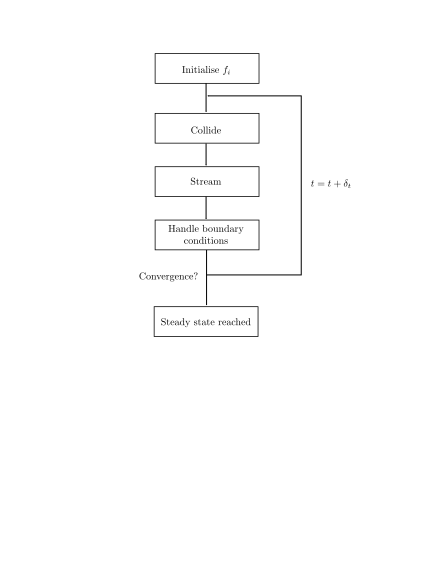
\includegraphics[width=0.5\textwidth]{fig/algorithm.pdf}
\end{center}
\caption[Flowchart of the most fundamental parts in an implementation
  of the LBM.]{Flowchart of the most fundamental parts in an implementation
  of the LBM. The convergence is usually tested for a macroscopic
  variable.}
\label{fig:lbm:algo}
\end{figure}

\nomenclature{LBE}{Lattice-Boltzmann Equation}


\section{The BGK collision operator}\label{sec:lbm:col}
The collision term in the LBE is the main ingredient in what
determines the physics of the system that is being modelled. Here the
desired interaction of the pseudo particles is stated. In section
\ref{sec:lbm:stat}, two necessary properties to approximations of the
full collision integral was stated.

One of the simplest collision operators that fulfil conditions (1)
and (2) in section \ref{sec:lbm:stat} is the BGK operator (BGK from
its creators: Bhatnagar, Gross and Krook). It was proposed in 1954 and
is today one of the most commonly used collision operators both in the
case of the lattice-Boltzmann and the continuous Boltzmann
equation. It is based on the principle of relaxing $f$ towards a
Maxwellian distribution. The relaxation is also performed in such a
way that the collision invariants are preserved.  In the discrete case,
eq. \eqref{eq:lbm:lbe}, the operator is given by:

\begin{equation}\label{eq:lbm:bgk}
\Omega_{ij} = \Omega_i = -\omega \left[ f_i(\x, t) - f_i^{(eq)}(\x, t)
  \right]
\end{equation}
where $\omega$ is a parameter determining the relaxation rate and
$\feq$ should be an equilibrium distribution that makes sure that the
necessary conditions are fulfilled. In the discrete case, a truncated
expansion of eq. \eqref{eq:lbm:maxwell} is typically used
\cite{wolf-gladrow}. This gives for instance


\begin{equation}
\feq = w_i\rho \left [ 1 + \frac{\ci \cdot \ubf}{c_s^2} +
  \frac{(\ci \cdot \ubf)^2}{2c_s^4} - \frac{\ubf^2}{2c_s^2} \right]
\end{equation}
where $w_i$ is a lattice specific weight, $\rho$ is the zeroth moment
of $\fii$ and $\ci$ is a unit velocity in the discretised velocity
space.

The BGK operator is due to its simplicity both when it comes to
theoretical treatment and implementation a popular choice. However in
some physical situations, e.g. multi-phase or high Reynolds-number
flows, more sophisticated alternatives are required
\cite{wolf-gladrow}. Throughout this work, the BGK operator will be
used.

\nomenclature{BGK}{Relaxation type collision operator (Bhatnagar,
  Gross and Krook)}


\section{The lattice}\label{sec:lbm:lattice}
symmetry... multi speed... weights ... D2Q9

\begin{equation}\label{eq:lbm:weights}
w_i = 
\left\{
  \begin{array}{l l}
    4/9 & \quad \text{if $i = 0$}\\ 
    1/9 & \quad \text{if $i = 1,2,3,4$}\\    
    1/36 & \quad \text{if $i = 5,6,7,8$}\\
  \end{array} \right.
\end{equation}

\begin{equation}\label{eq:lbm:d2q9_c}
\{\ci\} = \left\{
\begin{bmatrix}0\\0\end{bmatrix}, 
\begin{bmatrix}1\\0\end{bmatrix}, 
\begin{bmatrix}0\\1\end{bmatrix}, 
\begin{bmatrix}-1\\0\end{bmatrix}, 
\begin{bmatrix}0\\-1\end{bmatrix}, 
\begin{bmatrix}1\\1\end{bmatrix}, 
\begin{bmatrix}-1\\1\end{bmatrix}, 
\begin{bmatrix}-1\\-1\end{bmatrix}, 
\begin{bmatrix}1\\-1\end{bmatrix}
\right\} 
\end{equation}

\begin{figure}
  \centering
  \subfloat[D2Q7
    ]{\label{fig:lbm:h1}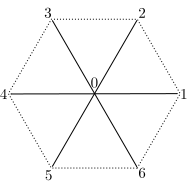
\includegraphics[width=0.47\textwidth]{fig/lattice_d2q7.pdf}}      
  \hspace{5pt}
  \subfloat[D2Q9
    ]{\label{fig:lbm:h2}\includegraphics[width=0.45\textwidth]{fig/lattice_d2q9.pdf}} 
  \caption{Two different unit cells for lattices used in the LBM in two
    dimensions. In (a) the D2Q7 seven speed lattice is shown and in
    (b) the nine speed D2Q9 lattice. The numbering at the edges is the
    usual naming convention for the different velocities.}
  \label{fig:lbm:lattices}
\end{figure}


\section{Asymptotic analysis}\label{sec:lbm:asym}
Methods from asymptotic analysis will, in this section, be used to
investigate the macroscopic limit of the general LBE. More detailed and
specific analyses for the three different equations considered will be
presented in sections \ref{sec:lbm:asym_np}, \ref{sec:lbm:asym_ns} and
\ref{sec:lbm:asym_pe} respectively. 

Asymptotic analysis is basically about describing mathematical objects
in some limit, e.g. how a function behaves for large or small values
of some variable or parameter. Consider for example the series $S_{\ep}$:

\begin{equation}
S_{\ep} = a^{(0)} + a^{(1)}\epsilon + a^{(2)}\epsilon^2 +
a^{(3)}\epsilon^3 + \mathcal{O}(\epsilon^4)
\end{equation}
It is clear that for sufficiently small values of $\epsilon$, the
terms of higher order is of negligible magnitude to those of lower
order and the series may be truncated at some point and still be a
good approximation of $S_{\ep}$. For example if $\ep$ is small, then
$S_{\ep} \approx a^{(0)}$ and we say that if $a^{(1)} \neq 0$ that
this approximation is of first order accuracy.

There are different approaches to go from the discrete LBE to a
continuous macroscopic equation. The most frequently applied one to
obtain the Navier-Stokes equations is the Chapman-Enskog method
\cite{junk-boundary}, which will reproduce the compressible
equations. Another method, often employed by M. Junk and his
associates, e.g. in \cite{junk-asym}, is a method based on regular
asymptotic expansions, this is also the method that will be utilised
in this work and will in the case of Navier-Stokes reproduce the
incompressible equations. A brief discussion of the differences
between the Chapman-Enskog and the regular expansion approaches will
be carried out at the end of this chapter.

The basic idea behind the analysis is to expand the distribution
function $\fii$ in some small parameter, $\epsilon$. Also this
parameter will be related to the spatial and time scales. The
macroscopic limit is obtained by taking the Taylor expansion of the
discrete LBE and comparing terms of equal order in
$\epsilon$. Together with the fact that certain quantities are
invariant under collisions, macroscopic differential equations are
obtained. Now follows the part of the analysis which is common for the
three equations, the more equation specific analysis is carried out in
sections \ref{sec:lbm:asym_np}, \ref{sec:lbm:asym_ns} and
\ref{sec:lbm:asym_pe} respectively.

\subsection{Motivation of the choice of expansion parameter}
A most desired property of the expansion parameter is that it should
be a small and dimensionless number. If the lattice is dense enough with
respect to the characteristic length scale of the system, a suitable
choice is the Knudsen number, $\ep$, which is defined as the ratio of
the mean free path, $\delta_x$, and the characteristic length of the
system under consideration, $\ell_0$, i.e. $\epsilon = \delta_x
/\ell_o$. To be able to perform the asymptotic analysis we must also
relate the time scale to this parameter. From the fact that the
lattice speed $c = \delta_x/\delta_t$ and by introducing a
characteristic speed, $u_o = \ell_0/t_0$, we have

\begin{equation}\label{eq:lbm:rel}
\epsilon = \frac{\delta_x}{\ell_0} = \frac{c}{u_0}\frac{\delta_t}{t_0}
\end{equation}
It is now clear that what determines the relation between the
timescale and the parameter $\epsilon$ is the ratio of the
characteristic speed and the lattice speed which is usually referred
to as the Mach number, Ma. In our particular case we will operate in
the incompressible limit, i.e. Ma $\ll$ 1 and a suitable choice is a
small number, thus Ma = $\epsilon$ is chosen \cite{junk-boundary}. The
discretisation of the space and time step is then related through

\begin{equation}
\delta_x'^2 = \delta_t' = \epsilon^2
\end{equation}
where the primes denote dimensionless variables. This particular
scaling is usually referred to as diffusive scaling.

\subsection{Expanding the LBE}
The LBE, eq. \eqref{eq:lbm:lbe}, with dimensionless variables and the
BGK collision operator reads:

\begin{equation}\label{eq:lbm:nodim_lbe}
f_i(\x' + \epsilon \cbf_i', t' + \epsilon^2) - f_i(\x', t') = -\omega \left[
  f_i(\x', t') - f_i^{(eq)}(\x', t') \right].
\end{equation} 
The primes denoting dimensionless variables will, for readability
reasons, from hereon be dropped. If nothing else is stated we always
consider dimensionless variables.

To obtain a differential equation, the difference equation in
eq. \eqref{eq:lbm:nodim_lbe} is Taylor expanded, which gives

\begin{equation}\label{eq:lbm:taylor_lbe}
\ep(\pd\fii) + \ep^2 (\partial_t\fii + (\pd \fii)^2/2 ) + \ep^3
(\partial_t (\pd\fii) + (\pd\fii)^3/6) + \bigO{\ep^4} = 
-\omega \left[
  f_i - f_i^{(eq)} \right]
\end{equation}
Expanding also $\fii$ and $\feq$ in the parameter $\epsilon$:

\begin{equation}\label{eq:lbm:fi_exp}
\fii = \fie{0} + \ep\fie{1} + \ep^2\fie{2} + \ep^3\fie{3} + \bigO{\ep^4}
\end{equation}

\begin{equation}\label{eq:lbm:fi_eq_exp}
\feq = \feqe{0} + \ep\feqe{1} + \ep^2\feqe{2} + \ep^3\feqe{3} +
\bigO{\ep^4}
\end{equation}
and inserting these expressions into eq. \eqref{eq:lbm:taylor_lbe}
gives an equation with terms of varying orders of $\ep$. Separating
this equation in equations of common orders allows for an analysis of
what happens at different scales of $\epsilon$. For the four leading
orders in $\ep$ we have:

\begin{equation}\label{eq:lbm:ep0}
\ep^0:\;\; 0 = -\omega \left[
  \fie{0} - \feqe{0} \right],
\end{equation}

\begin{equation}\label{eq:lbm:ep1}
\ep^1:\;\; \pd\fie{0} = -\omega \left[
  \fie{1} - \feqe{1} \right],
\end{equation}

\begin{equation}\label{eq:lbm:ep2}
\ep^2:\;\; \pd\fie{1} + \partial_t\fie{0} + (\pd \fie{0})^2/2 =
-\omega \left[ \fie{2} - \feqe{2} \right]
\end{equation}
and
\begin{equation}\label{eq:lbm:ep3}
\ep^3:\;\; \pd\fie{2} + \partial_t\fie{1} + (\pd \fie{1})^2/2 +
\partial_t (\pd\fie{0}) + (\pd\fie{0})^3/6 = -\omega \left[ \fie{3} -
  \feqe{3} \right].
\end{equation}

The idea is now that for an equation of a particular order in $\ep$,
use collision invariants and eliminate unknown $\fie{n}$ by using
equations of lower order in $\ep$. This will in the end, result in
differential equations for macroscopic variables, given by moments of
the $\fii$:s.

\nomenclature{CE, C-E}{Chapman-Enskog}


\section{LBM for the Nernst-Planck equation} 
The method presented here is based on representing the Nernst-Planck
equation, eq. \eqref{eq:et:np}, as an equation of advection-diffusion
type. Considering the quantity:  

\begin{equation}
\bar{\ubf} = \ubf -
  \frac{zq_eD}{k_BT}\nabla\psirm
\end{equation}
as an effective advective velocity, we have:

\begin{equation}\label{eq:lbm:adv-dif}
\dfrac{\partial \rho}{\partial t} + \nabla \cdot ( \bar{\ubf} \rho -
  D\nabla \rho ) = 0
\end{equation}
which is a mass conservation equation with fluxes from diffusion and
from advection respectively. The letter $\C$ for denoting the charge
concentration has in this section been replaced by the letter $\rho$
for avoiding the risk of confusing it with the lattice velocities
which traditionally are denoted by ${\ci}$.

A collision operator of BGK type, eq. \eqref{eq:lbm:bgk} will be used
together with a D2Q9 lattice. The lattice-Boltzmann equation then
reads:

\begin{equation}
f_i(\x + \cbf_i\delta_t, t + \delta_t) - f_i(\x, t) = -\omega \left[ f_i(\x, t) - f_i^{(eq)}(\x, t) \right]
\end{equation}
with $\{\cbf_i\}$ for the D2Q9 lattice as in
eq. \eqref{eq:lbm:d2q9_c}. The equilibrium function, $\feq$, is chosen
as \cite{alexey-tobias}:

\begin{equation}\label{eq:lbm:np_feq}
\feq = w_i \rho \left ( 1 + \frac{\ci \cdot \ubar}{c_s^2} \right)
\end{equation}
with the weights, $w_i$, as in eq. \eqref{eq:lbm:weights}. The charge
density and charge flux density is obtained by taking the zeroth and
first moments of the distribution function respectively, i.e:

\begin{equation}\label{eq:lbm:rho_mom}
\rho = \sum_i \fii
\end{equation}
and
\begin{equation}\label{eq:lbm:j_mom}
\jj = \sum_i \fii \ci
\end{equation}
The diffusion constant, $D$, is related to the relaxation parameter
$\omega$ through 

\begin{equation}
D = c_s^2 \left( \frac{1}{2} - \frac{1}{\omega} \right).
\end{equation}

\subsection{Asymptotic analysis}
To motivate the appearance of the above suggested method for solving
eq. \eqref{eq:lbm:adv-dif} and for showing under what premises the
method is valid, the macroscopic limit of the discrete scheme will
now be analysed in an asymptotic manner.

From the expansion of $\fii$ in eq. \eqref{eq:lbm:fi_exp} and from
eqs. \eqref{eq:lbm:rho_mom} and \eqref{eq:lbm:j_mom} follow the
expansions of the charge and flux density respectively as

\begin{equation}
\rho = \rhoe{0} + \ep\rhoe{1} + \ep^2\rhoe{2} + \ep^3\rhoe{3} + \bigO{\ep^4}
\end{equation} 
and

\begin{equation}
\jj = \je{0} + \ep\je{1} + \ep^2\je{2} + \ep^3\je{3} + \bigO{\ep^4}
\end{equation} 
The advective velocity is also expanded as: 

\begin{equation}
\ubar = \ubare{0} + \ep\ubare{1} + \ep^2\ubare{2} + \ep^3\ubare{3} + \bigO{\ep^4}
\end{equation}
By plugging these expansion into the equilibrium distribution
eq. \eqref{eq:lbm:np_feq}, the expansion in
eq. \eqref{eq:lbm:fi_eq_exp} is obtained. The terms of order zero is
used in the zeroth order equation of the LBE, eq. \eqref{eq:lbm:ep0},
which gives

\begin{equation}
\fie{0} = w_i\rhoe{0} \left( 1 + \frac{\ci \cdot \ubare{0}}{c_s^2} \right).
\end{equation}
However, since we are only considering the low Mach limit,
i.e. $|\ubar| \sim \ep$, we will in this analysis assume that
$\ubare{0} = 0$. And thus $\ubar$ will be of order $\ep$ to leading
order. It is possible to show \cite{junk-asymp} that if $\ubar$ is
initialised small it will also stay small if no major momentum sources
are present, thus it is a question of proper initialisation if the
assumption holds or not. Thus the expression for $\fie{0}$ reduces to

\begin{equation}
\fie{0} = w_i\rhoe{0}
\end{equation}




\section{LBM for the incompressible Navier-Stokes}\label{sec:lbm:ns}
The most frequent use of the LBM is to solve the Navier-Stokes
equations. In this work only the incompressible case,
eqs. \eqref{eq:et:ns_incompressible} and \eqref{eq:et:ns_mom} will be
considered. The LBM may however be used to reproduce weak
compressibility \cite{wolf-gladrow}. The incorporation of forces will
be treated in section \ref{sec:lbm:forces}. We recall the
incompressible Navier-Stokes equations without external forces present
from chapter \ref{sec:et} as:

\begin{equation}\label{eq:lbm:ns_inc}
 \nabla \cdot \ubf = 0
\end{equation}
and

\begin{equation}\label{eq:lbm:ns_mom}
\rhorm \left (\dfrac{\partial \ubf}{\partial t} +
  \ubf \cdot \nabla \ubf 
  \right ) = - \nabla \Prm  + \rhorm \nu \nabla^2 \ubf
\end{equation}
where $\nu$ is the kinematic viscosity related through the
dynamic viscosity, $\mu$, by

\begin{equation}
\mu = \rhorm \nu.
\end{equation}

A LBM will now be formulated for eqs. \eqref{eq:lbm:ns_inc} and
\eqref{eq:lbm:ns_mom}. The LBE with a BGK collision operator is given
by

\begin{equation}
f_i(\x + \cbf_i\delta_t, t + \delta_t) - f_i(\x, t) = -\omega \left[ f_i(\x, t) - f_i^{(eq)}(\x, t) \right]
\end{equation}
where

\begin{equation}\label{eq:lbm:ns_eq}
\feq = w_i\rho \left [ 1 + \frac{\ci \cdot \ubf}{c_s^2} +
  \frac{(\ci \cdot \ubf)^2}{2c_s^4} - \frac{\ubf^2}{2c_s^2} \right]
\end{equation}
where $w_i$ are the weights in eq. \eqref{eq:lbm:weights}.

The density, $\rhorm$, and the mass flux, $\rhorm \ubf$, is determined
from $\fii$ by taking the zeroth and first moments respectively:

\begin{equation}\label{eq:lbm:rho_mom}
\rhorm = \sum_i \fii
\end{equation}
and
\begin{equation}\label{eq:lbm:j_mom}
\rhorm \ubf = \sum_i \fii \ci .
\end{equation}
The kinematic viscosity is related to the relaxation parameter,
$\omega$

\begin{equation}\label{eq:lbm:nu}
\nu = c_s^2\left( \frac{1}{\omega} - \frac{1}{2} \right).
\end{equation}

\subsection{Asymptotic analysis}\label{sec:lbm:asym_ns}
Partially based on \cite{junk-asym}, an asymptotic analysis of the
above suggested method will be performed. In most literature
available, when reproducing the Navier-Stokes equations in the
macroscopic limit, a Chapman-Enskog expansion is performed. Note that
this is \emph{not} what is done here.

From the expansion of $\fii$ in eq. \eqref{eq:lbm:fi_exp} follows the
expansion of the macroscopic mass and velocity as

\begin{equation}\label{eq:lbm:ns_rho_exp}
\rho = \rhoe{0} + \ep\rhoe{1} + \ep^2\rhoe{2} + \ep^3\rhoe{3} +
\bigO{\ep^4}
\end{equation} 
and

\begin{equation}
\ubf = \ue{0} + \ep\ue{1} + \ep^2\ue{2} + \ep^3\ue{3} + \bigO{\ep^4}.
\end{equation}

These expansions are plugged into the equilibrium distribution in
eq. \eqref{eq:lbm:ns_eq} and from the equation of order zero in $\ep$,
eq. \eqref{eq:lbm:ep0} gives:

\begin{equation}
  \fie{0} = w_i \rhoe{0}
\end{equation}
Here $\ue{0}$ has been assumed to be zero by the same argumentation as
in the Nernst-Planck analysis, section
\ref{sec:lbm:asym_np}. Continuing to the equation of order 1 in $\ep$,
eq. \eqref{eq:lbm:ep1} and taking the first moment gives

\begin{equation}\label{eq:lbm:ns_rhoe0}
\nabla \rhoe{0} = 0.
\end{equation}
Further, by using this fact that $\rhoe{0}$ is constant in space and
that

\begin{equation}
\fie{1} = - \frac{1}{\omega} \pd\fie{0} + \feqe{1}
\end{equation}
where

\begin{equation}
\feqe{1} = w_i\left[ \rhoe{1} + \rhoe{0}\frac{\ci \cdot \ue{1}}{c_s^2}
  \right]
\end{equation}
gives when taking the zeroth moment of the equation of order two in $\ep$,
eq. \eqref{eq:lbm:ep2}

\begin{equation}
\partial_t \rhoe{0} + \nabla \cdot (\rhoe{0} \ue{1}) = 0.
\end{equation}
This equation states the conservation of mass for $\rhoe{0}$. Since
we are considering only systems in the incompressible limit,
$\rhoe{0}$ will be assumed to also be constant in time and we have

\begin{equation}\label{eq:lbm:ns_nodivu}
\nabla \cdot \ue{1} = 0.
\end{equation}
Taking the first moment of eq. \ref{eq:lbm:ep2} gives 

\begin{equation}\label{eq:lbm:ns_rhoe1}
\nabla \rhoe{1} = 0.
\end{equation}
It can be showed \cite{junk-asym} that if $\rhoe{1}$ is initialised
properly, then it does not change in time. Therefore, if $\rhoe{1}$ is
initialised to zero, it will also remain zero for all time.

As we now continue to the equation of order three in $\ep$, things
will get a bit more technical as we will make use of the fourth order lattice isotropy, eq. \eqref{eq:lbm:i4}. The zeroth moment of the equation gives

\begin{equation}
\nabla \cdot \ue{2} = 0.
\end{equation}
which may be used to show that $\ue{2} = 0$ \cite{junk-asym}, it will
not be shown here. Instead we continue by taking the first moment of
the equation, as it gets a bit more technical now, some intermediate
steps in the calculation will explicitly be written out. First from
the equation of order two in $\ep$ we have that

\begin{equation}
\fie{2} = -\frac{1}{\omega} \pd \fie{1} - \frac{1}{\omega} \partial_t
\fie{0} - \frac{1}{2\omega} (\pd \fie{0})^2 + \feqe{2}
\end{equation}
where

\begin{equation}
\feqe{2} = w_i \left[ \rhoe{2} + \rhoe{0} \frac{(\ci \cdot
    \ue{1})^2}{2c_s^4} - \rhoe{0} \frac{\left(\ue{1}\right)^2}{2c_s^2} \right]
\end{equation}
where the fact that $\ue{2} = 0$ have been used. Inserting the
expression for $\fie{2}$ into eq. \eqref{eq:lbm:ep3} gives, in index
notation

\begin{equation}\label{eq:lbm:foo1}
\begin{aligned}
\cc{\alpha}\cc{\beta}\parti{\beta} \left[ - \frac{\rhoe{0}}{\omega
    c_s^2} \cc{\gamma}\parti{\gamma}\cc{\delta} \uc{\delta} +
  w_i\rhoe{2} +
  \frac{\rhoe{0}w_i}{2c_s^4}\left(\cc{\gamma}\cc{\delta}\uc{\gamma}\uc{\delta}
  - (\uc{})^2 \right) \right] + \\ + \partial_tw_i\rhoe{0}\uc{\alpha} +
\frac{\rhoe{0}}{2 c_s^2}
\cc{\alpha}\cc{\beta}\parti{\beta}\cc{\gamma}\parti{\gamma}\cc{\delta}
= 0
\end{aligned}
\end{equation}
For brevity, the terms that in the end will equal zero have been
omitted. The indices $\alpha, \beta, \gamma$ and $\delta$ may take the
$x$ or $y$ component respectively. Summing eq. \eqref{eq:lbm:foo1}
over the directional index $i$ and by using the isotropity properties
of the lattice, eq. \eqref{eq:lbm:i0} gives:

\begin{equation}\label{eq:lbm:dino}
\begin{aligned}
c_s^2\rhoe{0}\left( \frac{1}{2} - \frac{1}{\omega}
\right)\parti{\beta} \left( \deltasec \right) + c_s^2\parti{\beta}\dab
\rhoe{2} +\\ + \frac{\rhoe{0}}{2}\left(( \deltasec) \uc{\gamma}\uc{\delta} -
\dd{\alpha}{\beta}(\uc{})^2 \right) + \rhoe{0}\partial_t \uc{\alpha} = 0
\end{aligned}
\end{equation}
On the form it is written now, it is not totally clear whether the
above equation is the incompressible Navier-Stokes momentum equation
or not. A simplification is in order and for brevity only the
simplification of one term is shown here.

By noting that $(\uc{})^2$ may be written as
$\dd{\gamma}{\delta}\uc{\gamma}\uc{\delta}$ we have

\begin{equation}
\begin{aligned}
 \parti{\beta}\left[ (\deltasec) \uc{\gamma}\uc{\delta} - \dd{\alpha}{\beta}(\uc{})^2\right] =
  \\ =\parti{\beta}\left[(\dd{\alpha}{\beta}\dd{\gamma}{\delta}+
  \dd{\alpha}{\gamma}\dd{\beta}{\delta})\uc{\gamma}\uc{\delta}\right]
\end{aligned}
\end{equation}
and by summing over $\gamma$ and $\delta$ the above expression reduces
to:

\begin{equation}
\parti{\beta} \left[ \uc{\alpha}\uc{\beta} + \uc{\beta}\uc{\alpha}
  \right] = 2\parti{\beta}\uc{\alpha}\uc{\beta} 
\end{equation}
and from incompressibility ($\parti{\beta}\uc{\beta} = 0$),
eq. \eqref{eq:lbm:ns_nodivu} we end up with

\begin{equation}
2\uc{\beta}\parti{\beta}\uc{\alpha}.
\end{equation}
By analogous simplification of the remaining terms in
eq. \eqref{eq:lbm:dino} we get

\begin{equation}\label{eq:lbm:ns_mom_index}
\rhoe{0} \left( \partial_t \uc{\alpha} +
\uc{\beta}\parti{\beta}\uc{\alpha} \right) = -\parti{\beta}(c_s^2
\rhoe{2}) + \rhoe{0}\nu \parti{\beta} \left( \parti{\beta}\uc{\alpha} +
\parti{\alpha}\uc{\beta} \right)
\end{equation}
where $\nu$ is defined as in eq. \eqref{eq:lbm:nu}, and if the
quantity $c_s^2\rhoe{2}$ is interpreted as the pressure, the above
equation is indeed the incompressible Navier-Stokes momentum equation,
eq. \eqref{eq:lbm:ns_mom}. It is satisfied by $\ue{1}$ in the
expansion of $\ubf$, since $\ue{2} = 0$, the error will be of order
$\ep^3$ and we say that the LB formulation is of second order accuracy
in velocity. $\rhoe{0}$ satisfies the mass equation and since
$\rhoe{1} = 0$ we say that the method is second order in density as
well \cite{junk-asym}. Since the pressure is included as a term in the
density expansion, problems with keeping the incompressibility might
arise if large enough pressures are present.

\subsection{Forcing schemes}\label{sec:lbm:forces}
Several methods have been proposed to add the forcing term in
eq. \eqref{eq:et:ns_mom} to the LBE. In \cite{krafczyk} five of these
methods have been compared. To briefly summarise the article; for
single phase flows, the methods achieve comparable. 

Due to its simplicity, a method formulated by Shan and Chen
\cite{shan-chen} was used in this work. It consists of modifying the
equilibrium distribution by computing it with the modified velocity

\begin{equation}
\ubf^{(eq)} = \frac{1}{\rho}\left(\sum_i \fii \ci +
\frac{\F\delta_t}{\omega} \right)
\end{equation}
where $\F$ is the external force. The physical velocity, $\ubf$, is
computed by

\begin{equation}
\ubf = \frac{1}{\rho}\left(\sum_i \fii \ci +
\frac{\F\delta_t}{2} \right).
\end{equation} 


\section{LBM for Poisson's equation}
As Poisson's equation, eq. \eqref{eq:pb}, is considered, a fundamental
difference to the Nernst-Planck and Navier-Stokes equations is
imediatley noted. It is not a differential equation of parabolic but
of elliptic type. If we consider what has been said about the LBM so
far in this chapter, it seems that it is a method that deals with
parabolic equations and not elliptic. However, by introducing a time
derivative to the Poisson's equation and only considering the steady state
solution the LBM may be used even for this equation. A diffusion-like
equation with a source term is then obtained

\begin{equation}\label{eq:lbm:poi_dif}
\partial_t\rho + \nabla^2 \rho = \R
\end{equation}
where $\R$ is the right-hand side of the Poisson's equation.

A LBM for this equation will now be formulated. The LBE to be solved
in this case is, an equation of the form:

\begin{equation}
f_i(\x + \cbf_i\delta_t, t + \delta_t) - f_i(\x, t) = -\omega \left[
  f_i(\x, t) - f_i^{(eq)}(\x, t) \right] + \Gi(\R)
\end{equation}
where $\Gi(\R)$ is an addition to the BGK collision operator to account
for the source term $\R$ in eq. \eqref{eq:lbm:poi_dif}. The equilibrium
distribution is given by

\begin{equation}
\feq = w_i \rho
\end{equation}
where $w_i$ are the weights in eq. \eqref{eq:lbm:weights}.

The quantity $\rho$ which in this work is interpreted to electric
potential in the steady state is determined by

\begin{equation}
\rho = \sum_i \fii
\end{equation}
and the quantity which, to us, is of even more interest, i.e. the
electric field, is given by

\begin{equation}
\nabla \rho = - \frac{\omega}{c_s^2 \delta_x} \sum_i \fii \ci.
\end{equation}
Finally, the addtional source term in the collision operator, $\Gi(\R)$,
is given by

\begin{equation}\label{eq:lbm:gi}
\Gi(\R) = w_ic_s^2 \left( \frac{1}{2} - \frac{1}{\omega} \right)\R.
\end{equation}

\subsection{Asymptotic analysis}\label{sec:lbm:asym_pe}
The given method for solving eq. \eqref{eq:lbm:poi_dif} will now be
motivated by preforming an asymptotic analysis of the suggested LBE.

$\fii$ is expanded as in eq. \eqref{eq:lbm:fi_exp} which gives an
expansion of $\rho$ as in eq. \eqref{eq:lbm:rho_exp}. Further, 
the source term $\R$ is expanded: 

\begin{equation}\label{eq:lbm:R_exp}
\R = \Rexp{0} + \ep\Rexp{1} + \ep^2\Rexp{2} + \ep^3\Rexp{3} + \bigO{\ep^4}
\end{equation} 
which also gives an expansion for the LBE source term as

\begin{equation}\label{eq:lbm:G_exp}
\Gi = \Gie{0} + \ep\Gie{1} + \ep^2\Gie{2} + \ep^3\Gie{3} + \bigO{\ep^4}.
\end{equation} 

The equilibrium distribution is expanded by plugging in the expansion
of $\rho$ from eq. \eqref{eq:lbm:rho_exp}. This gives for the zeroth
order equation in $\ep$, eq. \eqref{eq:lbm:ep0} that

\begin{equation}
\fie{0} = w_i\rhoe{0} + \frac{1}{\omega}\Gie{0}
\end{equation}
However, taking the first moment of the equation gives $\Gie{0} = 0$
and the above expression for $\fie{0}$ reduces to

\begin{equation}
\fie{0} = w_i\rhoe{0}.
\end{equation}

Coninuing to the equation of first order in $\ep$,
eq. \eqref{eq:lbm:ep1} and taking the zeroth moment gives that also
$\Gie{1} = 0$. Taking the first moment of the same equation  gives

\begin{equation}
\nabla \rhoe{0} = - \frac{\omega}{c_s^2} \sum_i \fie{1} \ci \approx -
\frac{\omega}{c_s^2 \delta_x} \sum_i \fii \ci
\end{equation}
Here, for the approximation, the expansion of $\fii$ is used together
with the fact that $\ep = \delta_x$ in dimensionless variables.

The next equation in $\ep$, i.e. the one of order two, will
eventually give us what we are looking for. Taking the zeroth moment
gives

\begin{equation}
-\frac{c_s^2}{\omega} \nabla^2 \rhoe{0} + \partial_t \rhoe{0} +
\frac{c_s^2}{2}\nabla^2 \rhoe{0} = \sum_i \Gie{2}(\Rexp{2})
\end{equation}
From this equation, it is deduced that in order to obtain Poisson's
equation in a steady state situation, i.e. when $\partial_t \rhoe{0} =
0$ the right-hand side must fulfill the follwong condition

\begin{equation}
\sum_i \Gie{2}(\Rexp{2}) = c_s^2\left( \frac{1}{2} - \frac{1}{\omega} \right)\Rexp{2}
\end{equation}
One such $\Gie{2}(R)$ is the one described in eq. \eqref{eq:lbm:gi}. 


\section{Algorithm/Scheme for solving the coupled equations}
In this section, the scheme to solve the coupled Poisson's,
Nernst-Planck and Navier-Stokes equations is described. The
dependencies between the equations are shown in
fig. \ref{fig:coupling}.

Following an initialisation of
the velocity field and charge density, an iteration in time is
performed. At each time step, a potential and electric field is
computed by solving Poisson's equation for the present charge
density. This is followed by updating the charge density from the new
potential and then the velocity field is updated with the prescence of
a force related to the charge density. The main ingredients in the
iterative algorithm are shown in fig. \ref{fig:lbm:full_algo}. 

\begin{figure}
\begin{center}
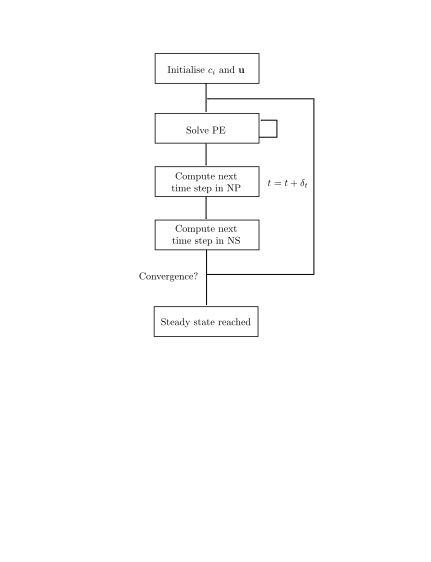
\includegraphics[width=0.4\textwidth]{fig/full_algorithm.pdf}
\end{center}
\caption{Flow scheme of the algorithm for solving the coupled equations.}
\label{fig:lbm:full_algo}
\end{figure}


\section{Boundary conditions}\label{sec:lbm:bound}
In all physical situations, when solving a differential equations on a
domain, conditions for what is happening on the boundary of the domain
must be specified. So far, only the update rule for $\fii$ on the
interior of this domain has been treated. In this section we will
also define rules for the boundaries of the domain. The nodes in the
interior and the boundary will be referred to as \emph{interior nodes}
and \emph{boundary nodes} respectively. Typically, a boundary
condition in a macroscopic variable, e.g. velocity, is specified from
the physical problem. This condition must be translated into a
condition for the distribution function, $\fii$, on the statistical
level. In this section some, to this work, useful boundary conditions
will be formulated and discussed.

\begin{figure}
\begin{center}
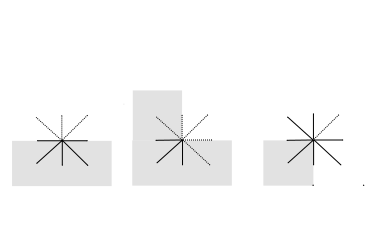
\includegraphics[width=0.9\textwidth]{fig/bb.pdf}
\end{center}
\caption[Three different boundary situations in the LBM.]{Three
  distinct boundary situations that in general has to be treated
  differently. From left to right, a straight boundary, a corner and
  an edge. Grey areas are outer of the domain. The solid arrows
  corresponds to known directions of the distribution function and
  dotted lines to unknown.}
\label{fig:lbm:bounds}
\end{figure}

\subsection{Bounce-back boundaries}\label{sec:lbm:bb}
The lattice-Boltzmann approach is often praised for its rather
straight-forward easiness of implementing boundary conditions. One of
the simplest and most commonly used is the bounce-back rule. It is a
mesoscopic rule for implying a Dirichlet condition on the first
moment. In the case of specifying boundary conditions for
Navier-Stokes, it may be used to set a velocity at a boundary,
typically at wall boundaries the velocity is set to zero.

The bounce-back rule for setting the first moment to zero reads

\begin{equation}
\fii^{(bb)} = f_{i^*}
\end{equation}
where $\mathbf{c}_{i^*}$ is the direction opposite to $\ci$. This
justifies the name of the rule, all pseudo particles are propagated in
a direction opposite to where they came from, i.e. bounced back. If
the boundary nodes are updated between the collision and streaming
step, all directions should be updated with its opposite
counterpart. However, if the update is performed after the streaming
step, only the unknown directions are to be updated, see
fig. \ref{fig:lbm:bounds}. These two schemes are referred to full-way
and half-way bounce-back. If a non-zero Dirichlet condition is
desired, it is possible to add some momentum to suitable directions.

It is possible to show that, in the case of a straight boundary, the
actual boundary is with second order accuracy located half a node-node
distance into the computational domain \cite{junk-boundary}. Thus, the
boundary will not be located at the boundary node. 

As suggested earlier in this section, this type of local boundary
conditions allows for easy implementation of more or less arbitrary
boundaries. In fig. \ref{fig:lbm:cool_flow}, an example of 2D flow in a
complicated domain is shown. At the walls in the figure, bounce-back
conditions are used.

\begin{figure}
\begin{center}
\includegraphics[width=0.9\textwidth]{fig/comp_bound_u.pdf}
\end{center}
\caption[Example of flow in a non-trivial geometry.]{Example of flow
  in a non-trivial geometry where bounce-back boundaries are used.}
\label{fig:lbm:cool_flow}
\end{figure}

\subsection{Slip boundaries}\label{sec:lbm:mirror}
A zero friction (slip) boundary condition may be imposed by the
following rule for the straight boundary situation in
fig. \ref{fig:lbm:bounds}. Instead of making all pseudo particles
``bounce back'', they are reflected in a mirror-like manner, see
fig. \ref{fig:lbm:slip}. This gives that the component normal to the
boundary of the first moment is zero while the tangential component is
unchanged. In this work, this condition is used to set the
ion flux through the boundary to zero, eq. \eqref{eq:et:j0}.

It is not as straight-forward to define rules at corner and edge
nodes, as for the straight boundary nodes. From tests, it has been
shown that adequate accuracy may be obtained by treating the corner or
edge as two perpendicular straight boundaries and mirror reflect half
of the distributions at each plane respectively. 

\begin{figure}
  \centering
  \subfloat[Bounce-back
    ]{\label{fig:lbm:no_slip}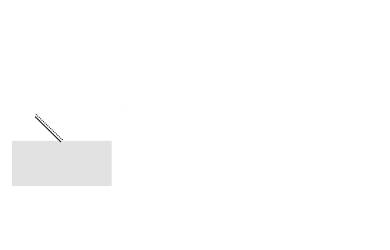
\includegraphics[width=0.35\textwidth]{fig/no_slip.pdf}}      
  \hspace{5pt} \subfloat[Mirror reflection
  ]{\label{fig:lbm:slip}\includegraphics[width=0.35\textwidth]{fig/slip.pdf}}
  \caption[Intuitive scheme for the bounce-back and mirror reflection
    conditions.]{Intuitive scheme for an incoming pseudo particle for
    two common boundary conditions in the LBM. The bounce-back rule
    (a) and mirror reflection (b).}
  \label{fig:lbm:bbs}
\end{figure}

\subsubsection{With momentum addition}\label{sec:lbm:mod_mirror}
In the case with the fixed surface charge boundary condition,
eq. \eqref{eq:et:fix_c}, we do not wish to set the normal component to
zero but to some value of the surface charge. This is realised by
adding some ``momentum'' in the three directions pointing in to the
domain. The total surface charge may be divided between the directions
in different proportions, in this work it is however evenly
distributed, i.e. one third per direction. 

%\subsection{he-zou, constant density/velocity}\label{sec:lbm:hezou}

%\subsection{Maybe something on non-local boundary conditions}


\section{Physical and lattice units}

A physical system may in its physical units contain quantities which
numerical values may differ a lot from each other. It is therefore
typically a very bad idea and in the case with lattice-Boltzmann it
will in general not work to just solve the equation in physical
units. The equation is therefore scaled to dimensionless form by
introducing characteristic quantities. For example a quantity A is
scaled by A$_0$ to a dimensionless quantity A' through

\begin{equation}
\mathrm{A}' = \mathrm{A}/\mathrm{A_0} 
\end{equation}


\section{Chapman-Enskog vs. regular expansion analysis}
When reading literature and articles about the LBM, different
approaches may be used to derive the macroscopic behaviour of the
LBM. The aim of this section is to bring some clarity and briefly
explain the main differences between two of these.

The method used in this work is referred to as regular (error)
expansion analysis \cite{junk-comparison} and is used with one time
scale. In the case of analysing the macroscopic behaviour of the LBM
for the Navier-Stokes equations, the incompressible equations are
obtained. The mass and momentum equations are exactly satisfied by
$\rhoe{0}$ and $\ue{1}$ from the regular expansions of $\rho$ and
$\ubf$ respectively.

An other approach is by using the so called Chapman-Enskog analysis
\cite{wolf-gladrow}. This is a traditional method in kinetic theory
and is the most frequently used in litterature about the LBM. Here two
time scales are used, on faster (convective) and one slower
(diffusive). This gives that in the macroscopic limit of the LBE, the
compressible Navier-Stokes equations are obtained. In the C-E analysis,
the full quantities $\rho$ and $\ubf$ are showed to satisfy, not the
exact, but the N-S equations with higher order error terms.


